\documentclass[oneside,12pt]{report}
\usepackage[latin1]{inputenc} 
\usepackage[T1]{fontenc}
\usepackage[frenchb]{babel} 
\usepackage{hyperref}
\usepackage[dvips]{graphicx}

\usepackage[usenames]{color}
\usepackage{tabularx}
\usepackage{colortbl}
\usepackage{float}
\usepackage{tikz}
\usepackage{indentfirst}
\usepackage{pgf}
\usepackage{pgfplots}
\usepackage{moreverb}
\usepackage{url}
\usepackage{babelbib}
\usepackage{multirow}
\sloppy
\usepackage{setspace}
\usepackage{algorithmic}
\usepackage{algorithm}
\usepackage{listings}
\usepackage{fancybox}
\usepackage{rotating}
\usepackage[strict]{changepage}
\usepackage{relsize}
\usepackage{geometry}
%\usepackage{latexsym}     
%\usepackage{makecell} 
%\usepackage{pdflscape}
%\usepackage{caption}
%\renewcommand{\cellalign}{cc}
%\renewcommand{\theadalign}{cc}

%%%%%%%%%%%%%%%%%%%%%%%%%%%%%%%%%%%%%%%%%%%%%%%%%%%%%%%%%%%
\usepackage[acronym]{glossaries}
%\usepackage{acronym}
%\usepackage{glossaries}
%\makeglossaries
%%%%%%%%%%%%%%%%%%%%%%%%%%%%%%%%%%%%%%%%%%%%%%%%%%%%%%%%%%%
\def\UrlBreaks{\do\/\do-}
\hypersetup{
backref={true}, %permet d'ajouter des liens dans...
pagebackref=true,%...les bibliographies
hyperindex=true, %ajoute des liens dans les index.
colorlinks=true, %colorise les liens
breaklinks=true, %permet le retour � la ligne dans les liens trop longs
citecolor=blue,
urlcolor= blue, %couleur des hyperliens
linkcolor= black, %couleur des liens internes
bookmarks=true, %cr�er des signets pour Acrobat
bookmarksopenlevel=1,
%bookmarksopen=true, %si les signets Acrobat sont cr�es,
%les afficher compl�tement.
pdftitle={}, %informations apparaissant dans
pdfauthor={}, %dans les informations du document
pdfsubject={} %sous Acrobat.
}

%%%%%%%%%%%%%%%%%%%%%%%%%%%%%%%%%%%%%%%%%%%%%%%%%%%%%%%%%%%%%%%%%
%*****************************************
% INTERLIGNE
%\renewcommand{\baselinestretch}{1.2}
%******************************************

%Fichier PDF interactif%%%%%%%%%%%%%
%\usepackage{color}
%\usepackage[colorlinks=true,urlcolor=blue]{hyperref}
%%%%%%%%%%%%%%%%%%%%%%%%%%%%%%%%%%%%
%[dvipdfm,colorlinks=true,urlcolor=blue,pdfhighlight =/O]
%\usepackage[english]{algorithme}
%\usepackage{layout}
%\DeclareFontFamily{T1}{cmr}{\hyphenchar\font=-1}
%------------------------------------------------------------
%\usepackage{times}
%-----------------------------------------------------------
%%%%%%%%%%%%%%%%%%%%%%%%%%%%%%%%%%%%%%%%%%%%%%%%%%%%%%%%%%%%
%Espace entre Legende et Texte
%\setlength\abovecaptionskip{10\p@}
%\setlength\belowcaptionskip{0\p@}
%%%%%%%%%%%%%%%%%%%%%%%%%%%%%%%%%%%%%%%%%%%%%%%%%%%%%%%%%%%%%
%-----------------------------------------------------------
% Profondeur de \subsubsection = 3
\setcounter{tocdepth}{3}     % Dans la table des matieres
\setcounter{secnumdepth}{4}  % Avec un numero.
%-------------------------------------------------------------------
%           Corrections pour les imprimantes recto-verso
%                          (A AJUSTER)
%-------------------------------------------------------------------
%\ShiftOddPagesRight{-1mm}
%\ShiftOddPagesDown{2.5mm}
%\ShiftEvenPagesRight{0mm}
%\ShiftEvenPagesDown{0mm}
%-------------------------------------------------------------------
%                             Marges
%-------------------------------------------------------------------
% pour positionner les vraies marges:
%\SetRealMargins{1mm}{1mm}
%-------------------------------------------------------------------
%                             En-tetes
%-------------------------------------------------------------------
\newcommand\upun[1]{\uppercase{\underline{\underline{#1}}}}
\FormatHeadingsWith\upun
\newcommand\itheadings[1]{\textit{#1}}
\FormatHeadingsWith{\itheadings}
\setlength{\HeadRuleWidth}{0.4pt}

%\parindent=2cm
\setlength{\parindent}{3ex}
%-------------------------------------------------------------------
%                         Les references
%-------------------------------------------------------------------
\NoChapterNumberInRef
\NoChapterPrefix
\makeglossary
\makeindex
%-----------------------------------------------------------------
%               Document
%-----------------------------------------------------------------
\begin{document}
\renewcommand{\bibname}{Bibliographie}
\renewcommand{\tablename}{Tableau}
\renewcommand{\contentsname}{Table des mati�res}
\renewcommand{\listtablename}{Liste des tableaux}
\renewcommand{\listfigurename}{Liste des figures}
\renewcommand{\chaptername}{Chapitre}
      \OddHead={{\leftmark\rightmark}{\hfil\slshape\rightmark}}
      \EvenHead={{\leftmark}{{\slshape\leftmark}\hfil}}
      \OddFoot={\hfil\thepage}
      \EvenFoot={\thepage\hfil}
      \pagestyle{ThesisHeadingsII}
\ResetChaptersAtParts 

%-------------------------------------------------------------------
%                         Page de titre:
%-------------------------------------------------------------------
\ThesisTitle{{ La m�thode GRASP (Greedy Randomized Adaptive Search Procedure) combin�e au Path Relinking pour la r�solution du probl�me d'affectation quadratique }}
\ThesisDate{2017}
\ThesisAuthor{ZEMRI Ahmed}
\ThesisUPS
% Jury
\President{******** }
\Rapporteurs{Mr L.LOUKIL & Universit� d'Oran 1}
%\Supervisor{}
\Examinateurs{************ & Universit� d'Oran 1 \\ *********** & Universit� d'Oran 1}
%\NewJuryCategory{supervisor}{\it  Directeur de th�se :}
                        %{\it  Directeur de thse :}
                       
                      \MakeThesisTitlePage
%-------------------------------------------------------------------
%                          remerciements
%-------------------------------------------------------------------
%\DontFrameThisInToc
\begin{ThesisAcknowledgments}
\vspace{1,5cm}
\bigskip
Ceci contient les remerciements .....


\bigskip
\end{ThesisAcknowledgments}
%-------------------------------------------------------------------
%                            dedicace
%-------------------------------------------------------------------
\begin{ThesisDedication}
%\LARGE
\vspace{1,5cm}
Je d�die ce travail,\\
A mes ch�res parents \\ 
A mes fr�res et s\oe urs \\


%\normalsize
\end{ThesisDedication}
%-------------------------------------------------------------------
%                  ecriture de `Chapitre'et `Partie'
%                      dans la table des matieres
%-------------------------------------------------------------------
\WritePartLabelInToc
\WriteChapterLabelInToc
%-------------------------------------------------------------------
%                        R�sum�
%-------------------------------------------------------------------


%-------------------------------------------------------------------
%                        table des matieres
%-------------------------------------------------------------------

\tableofcontents
\listoffigures  % table des figures
\listoftables  % table des tableaux
%\include{ACRONYMES}
\mainmatter
%\frenchspacing
%\printglossaries
%section sans numerotation
%\SpecialSection{Introduction}
%Titre de l'introduction: Contexte g�n�ral, Probl�matique et Objectifs
%--------------------------------------
% Chapitres
%--------------------------------------
%\newacronym{TEM}{TEM}{scanning electron microscope}
\begin{spacing}{1.2}
%%%%%%%%%%%%%\begin{spacing}{1.3} % pour une autre interligne

\chapter*{Introduction g�n�rale}

\chapter{cloud computing}
\section{introduction}

Le Cloud Computing, ou Informatique en nuages, est un paradigme qui a attir� une attention toute particuli�re ces derni�res ann�es dans le monde de l'informatique, il consiste � proposer les services informatiques sous forme de services � la demande, accessibles de n'importe o�, n'importe quand et par n'importe qui.
Dans ce chapitre nous allons pr�senter les notions fondamentales du Cloud Computing, ses enjeux, ses �volutions et son utilit� ainsi que la technologie qui la constitue et les diff�rents acteurs du secteur.
Nous devons dans un premier temps �tudier le Cloud Computing de mani�re g�n�rale (Ces origines ,D�finitions '),puis dans un second temps nous allons �tudier les trois services principaux, sur lesquels le Cloud Computing repose applicatif,plateforme, infrastructure(Saas,Paas,Iaas)et les modele de deploiment ,Et la derni�re partie de ce chapitre pr�sente les diff�rents acteurs principale de Cloud Computing.
\section{Concepts et technologies � l'origine du � Cloud Computing ��:}
Le Cloud Computing est la r�union de diff�rents concepts informatiques, �tudi�s et d�velopp�s depuis les ann�es 60, associ�s � certaines technologies, r�cemment accessibles financi�rement et matures techniquement. Dans la suite nous allons d�tailler 5 concepts et technologies qui nous semblent �tre fondamentaux pour  d�finir les fondements du cloud computing
\subsection{L'informatique utilitaire de John McCarthy�:}
Ce concept se base sur la notion de consommation et a �t� propos� en 1961,lors d'une conf�rence au MIT (Massachusetts Institute of Technology), par John McCarthy aussi connu comme l'un des pionniers de l'intelligence artificielle (dont il proposa le nom en 1955) et pour avoir invent� du LISP en 1958. Lors de ce discours, John McCarthy sugg�ra que la technologie informatique partag�e � time-sharing � pouvait construire un bel avenir dans lequel la puissance de calcul et m�me les applications sp�cifiques pouvaient �tre vendues comme un service public. Cette
id�e, tr�s populaire dans les ann�es 60, disparu au milieu des ann�es 70 : � l'�poque, les technologies mat�rielles, logicielles et r�seaux n'�taient tout simplement pas pr�tes. Le CC met en oeuvre l'id�e d'informatique utilitaire du type service public, propos�e par John McCarthy.
\subsection{Le concept de � grille informatique ��:}
ce concept est apparu en 1997 lors d'un s�minaire au laboratoire national d'Argonne intitul�
� Building a Computational Grid �,Le Grid Computing est une technique de calcul consistant � partager 
les ressources de tout �l�ment informatique permettant l'ex�cution d'une t�che ou le stockage d'une donn�e num�rique.
Les ressources informatiques de cette infrastructure virtuelle, reli�es de fa�on logique, sont d�localis�es et autonomes.
Cette technique permet de r�soudre des probl�mes que l'utilisation d'un super-ordinateur ne pourrait pas 
solutionner dans un temps r�aliste et fournir d'autre service comme debit,disponibilit�,s�curit�,
Il s'inspire grandement du concept de informatique utilitaire .
\subsection{Le concept de � ferme de serveurs ��:}
Les fermes de serveurs sont apparues au d�but des ann�es 2000 ,Ces � fermes � h�bergent jusqu'� plusieurs centaines de serveurs mont�s en Cluster.
Le � Clustering � est une technique qui consiste � regrouper plusieurs serveurs (ou � n�uds �) ind�pendants dans un m�me lieu afin de d�passer les limitations d'une machine unique. Les diff�rents n�uds mis en r�seau ensemble vont appara�tre comme une seule machine ayant plus de capacit�s plus de puissance, de m�moire, de stockage.
\subsection{Les fournisseurs de services d'application�:}
Les fournisseurs de services d'application ont aussi leur importance dans l'origine du � Cloud Computing �,Une ASP d�signe une application fournie comme un service ,Plut�t que d'installer le logiciel sur le poste client en ayant � assurer les phases d'installation et de maintenance sur chaque poste, les applications ASP sont h�berg�es et centralis�es sur un serveur unique et accessible par les clients au travers de protocole standard,comme par exemple le cas avec des applications Web accessibles par http�:il n'y a alors plus de d�ploiement ou de maintenance � effectuer sur le poste utilisateur, celui-ci n'a alors besoin que d'un simple navigateur Internet. Le d�ploiement, la configuration, la maintenance, la sauvegarde, etc. sont d�sormais de la responsabilit� du fournisseur du service, le client est alors consommateur.

On s'int�resse en notre travail � la deuxi�me probl�me.

\subsection{La virtualisation�:}
La virtualisation est un concept beaucoup plus ancien qui constitue le socle du Cloud Computing. La virtualisation regroupe l'ensemble des techniques mat�rielles ou logicielles permettant de faire fonctionner, sur une seule machine physique, plusieurs configurations informatiques (syst�mes d'exploitation, applications, m�moire vive,...) de mani�re � former plusieurs machines virtuelles qui reproduisent le comportement des machines physiques,Les premiers travaux peuvent �tre attribu�s � IBM,qui dans les ann�es 60, travaillait d�j� sur les m�canismes de virtualisation en d�veloppant dans les centres de recherche de Cambridge et de Grenoble, CMS (Conversation Monitor System), le tout premier hyperviseur. C'est donc depuis presque 50 ans que l'id�e d'une informatique � la demande est pr�sente dans les esprits m�me si les technologies n'�taient jusqu'alors pas au rendez-vous pour pouvoir concr�tiser cette id�e.
\section{D�finition�}
Il existe de nombreuses d�finitions du terme Cloud Computing (informatique dans le nuage) et il y a peu de consensus sur une seule et universelle d�finition,Cette multitude de d�finitions refl�te sur la diversit� et la richesse technologique du Cloud Computing.
Nous citons quelque difinition:
\begin{description}
 \item[cloud computing]: la d�finition propos�e par CISCO [2] : 'le Cloud Computing est une plateforme de mutualisation informatique fournissant aux entreprises des services � la demande avec l'illusion d'une infinit� des ressources'
\item pour Microsoft�:
L'ensemble des disciplines, technologies et mod�les commerciaux utilis�s pour d�livrer des capacit�s informatiques (logiciels, plates-formes,mat�riels), comme un service � la demande.
'Le service � la demande (vous ne payez que ce que vous utilisez);
'Le service est accessible n'importe o�;
'Le service est mesur�, ce qui permet de pr�server les ressources;
'La quantit� est modulable � la location (�lasticit� infinie !);
'Les ressources sont mises en commun, ce qui r�duit les co�ts.
\item
Pour EMC, Fournisseur de solutions d'archivage et de stockage : 
Le CloudComputing permet aux utilisateurs d'acc�der aux pools de ressources quand
ils le souhaitent et b�n�ficient ainsi de l'�fficacit� partag�e et de souplesse.
\item
Cependant, la d�finition propos�e par la National Institute of Standards and Technology
(NIST)[nist] est devenue la r�f�rence accept�e par le public. NIST d�finit le Cloud Computing comme �tant un mod�le qui permet l'acc�s via un r�seau d'une fa�on simple et � la demande � un ensemble des ressources informatiques mutualis�es et configurables (ex r�seaux, serveurs, stockage, applications et services). Ces ressources informatiques peuvent �tre allou�es et lib�r�es rapidement avec le minimum d'effort de gestion ou d'interaction avec les fournisseurs de services.

 \end{description}
%import les image 
\begin{center}
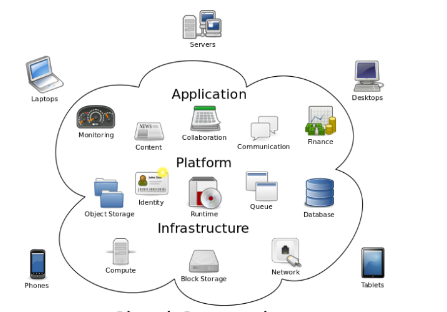
\includegraphics[scale=0.6]{Figures/cloud_computing.png}

\caption{figure: cloud computing}
\label{fig1}
\end{center}
\section{L'�volution de Cloud computing:}
Le Cloud computing est le fruit d'une �volution pouvant �tre pr�sent�e en 5 phases :
\begin{description}
 \item [*] Elle d�bute avec les Fournisseurs d'Acc�s Internet (FAI 1.0). Ils ont pour but de mettre en place des moyens de t�l�communication pour assurer le raccordement des personnes ou entreprises au r�seau internet.
 \item [*]La seconde phase est l'orientation des FAI vers l'h�bergement de pages web (FAI 2.0). Cette phase marque un grand bond dans le d�veloppement d'internet.
 \item [*] La troisi�me phase (FAI 3.0) est la possibilit� qu'offrent les FAI � h�berger des applications m�tiers des entreprises.
 \item [*] Une connaissance des besoins applicatifs des entreprises permettent aux FAI de faire �voluer leur domaine d'intervention. Ils mettent en place des plateformes de g�n�ration d'applications � la demande. Il s'agit des ASP (Application Service Provider) dont les "Software as a Service" sont des d�rives�:c'est le FAI 4.0.
 \item [*] La g�n�ralisation des pratiques pr�c�dentes, la prise en compte de nouvelles pratiques et l'int�gration des principes que nous pr�sentons dans les sections suivantes donnent naissance au cloud computing [Fos49].
 
\end{description}
\begin{center}
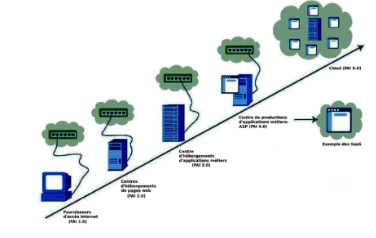
\includegraphics[scale=0.6]{Figures/evolution_de_cloud_computing.png}

\caption{figure: evolution de cloud computing}
\label{fig2}
\end{center}
\section{Les caract�ristiques essentielles de cloud computing�:}
\subsection{Self-service � la demande�:}
L'utilisateur d'un service de � Cloud Computing � a la capacit� (� self-provisioning �)
d'approvisionner lui-m�me de nouvelles ressources telles que de l'espace disque, des serveurs virtuels, du temps CPU, des nouvelles bo�tes aux lettres, '
\subsection{Elasticit� et rapidit�:}
Les ressources peuvent �tre allou�es ou d�sallou�es rapidement. C'est une des caract�ristiques essentielles du Cloud computing , la capacit� d'augmenter et de r�duire le volume des ressources utilis�es en fonction des besoins, de m�me que lib�rer les ressources qui ne sont plus n�cessaires, au profit d'autres utilisations,Ces op�rations peuvent se faire par demande ou de fa�on automatique,par
programmation ou triggers.
\subsection{Acc�s aux ressources�:}
Les ressources sont disponibles via le r�seau Internet, ou via l'Intranet dans le cas d'un Cloud priv�.
Les ressources sont accessibles via des protocoles standards (TCP/IP,SSL, HTTP,...)L'acc�s aux ressources peut se faire � partir d'un grand nombre de p�riph�riques clients (ordinateurs, portables, t�l�phones mobiles, smartphones, ...)et depuis n'importe quelle plate-forme (Windows, Unix, MacOs, Linux, syst�mes propri�taires,')
\subsection{Allocation des ressources�:}
Les ressources mises � disposition par les providers de � Cloud Computing � sont mutualis�es pour r�pondre aux besoins de plusieurs clients dans une architecture multi-tenant.
Une architecture  � multi-tenant � ou  � multi-locataire � fait qu'une seule instance d'une application est adapt�e aux besoins de tous les utilisateurs et offre malgr� tout un certain niveau de customisation pour s'adapter de mani�re individualis�en aux diff�rents clients.
\subsection{Mesure du service�:}
Toutes les ressources allou�es peuvent �tre surveill�es et contr�l�es de mani�re automatique et  optimise l'utilisation de ressources en s'appuyant sur le mod�le 'payez uniquement ce que vous consommez'.
\section{Taxonomie du cloud computing:}
Avant de pr�senter les diff�rents types de cloud pouvant �tre d�velopp�s, nous �tablissons dans un premier temps quelques crit�res de classification :
\begin{enumerate}
 \item {La raison de d�veloppement (business model):} c'est la raison qui justifie la mise en place de la plateforme. Elle peut �tre commerciale, scientifique ou communautaire...ex.
 \item {Le modele  de services�:}c'est le modele de service que peut �tre d�livr� par le cloud aux clients.
 \item { L'accessibilit� :}Le cloud peut �tre accessible par tous (``cloud public'') ou restreint � un public particulier (``cloud priv�''), C'est la raison qui justifie le d�ploiement de la plateforme de cloud.
\end{enumerate}
\subsection{ raison de d�veloppement�:}
L'utilisation du CC ne se limite pas uniquement aux entreprises � caract�re commercial. En fonction des raisons de sa mise en place, nous distinguons quatre cat�gories de plateformes de CC � savoir :
\begin{description}
 \item \textbf{Cloud d'Entreprises}�:Dans cette cat�gorie, nous retrouvons des entreprises de petites et de moyennes tailles disposant chacune de peu de ressources et de moyens de maintenance de leurs infrastructures. Elles se regroupent donc autour d'un projet de cloud afin de mutualiser leurs capacit�s.La plateforme qui en d�coule est priv�e, c'est-a-dire accessible uniquement
par les entit�s des diff�rentes entreprises. Cette plateforme � l'avantage d'�tre de petite taille et d'acc�s restreint � des utilisateurs connus.
\item \textbf{Cloud Gouvernemental et Recherche Scientifique�:}des instituts de recherche mettent leur pieds sur  des environnements de cloud pour des raison de recherche scientifique de developement ,L'acc�s est r�serv� aux personnes appartenant aux instituts de recherche associ�s.
\item \textbf{Cloud pour R�seaux Sociaux et Jeux�:}Le d�veloppement des r�seaux sociaux et des jeux en ligne n�cessite de plus en plus de grandes quantit�s de ressources.ca implique la  d�veloppement d'une plateforme similaire au cloud devient une �vidence pour optimiser l'utilisation des ressources et faciliter le partage de donn�es. En effet, elles sont consid�r�es
comme un cloud .
\item \textbf{Cloud pour Fournisseurs de Services�:}C'est le mod�le le plus r�pandu. Une entreprise, appel�e fournisseur, met � la disposition d'autres (appel�es clients) une plateforme d'ex�cution d'applications et assure le service informatique inh�rent.
\end{description}

\subsection{Le modele  de services:}
Le but principal du Cloud est d'offrir des services � des utilisateurs ,suivant diff�rents
mod�les.  NIST pr�cise que le Cloud Computing a trois mod�les de services principaux Iaas,Paas,Saas
\begin{center}
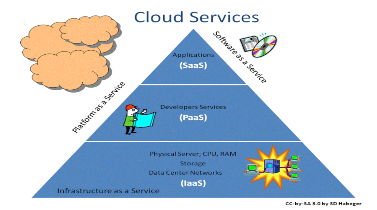
\includegraphics[scale=0.6]{Figures/modele_de_service.png}

\caption{figure : modele de srvice}
\label{fig2}
\end{center}

\begin{description}
 \item \textbf{Infrastructure en tant que service(infrastructure as a Service  ��Iaas��)�:}
 Dans ce mod�le, l'infrastructure physique (le mat�riel r�seau, le mat�riel serveur, la plate-forme de
virtualisation, les moyens et capacit�s de stockage) est � d�mat�rialis�e � et h�berg�e.
Le fournisseur procure donc une couche mat�rielle (serveurs, r�seau, stockage, hyperviseur, solution de supervision, solution de management) sur laquelle les clients vont pouvoir d�poser leurs environnements syst�me et leurs applications.
Mais ce service va encore plus loin gr�ce � la virtualisation. L'utilisation de cette technologie permet aux clients de cr�er leur propre infrastructure personnalis�e (serveurs virtuels, r�seau virtuel, stockage) en quelques clicks. Cette infrastructure est par ailleurs extr�mement flexible, accessible sans restriction et configurable en temps r�el.
Les clients n'ont pas � se soucier de la scalabilit� de leur infrastructure, cette t�che �tant g�r�e par le fournisseur. Celui-ci g�re �galement tous les co�ts de gestion li�s au fonctionnement du mat�riel (�lectricit�, climatisation, etc) ainsi que le contr�le de la consommation s'il y a une facturation � l'usage (au Go, au temps d'utilisation, etc).
Il y a un avantage principal dans ce niveau de service. Le client n'a plus � construire son propre Datacenter, ni � g�rer l'infrastructure physique et les co�ts qui lui sont inh�rents.
L'ing�nieur ou l'administrateur syst�me peut se reconcentrer sur l'optimisation de son
environnement syst�me, et le d�veloppeur sur ses applications. En fait, le client � un contr�le total de son Datacenter virtuel sans se soucier de son �lasticit�, ni de l'infrastructurephysique qu'il y a derri�re.
Mais ce mod�le a �galement des inconv�nients. D�j�, comme pour toute infrastructure informatique classique, il est indispensable d'avoir un administrateur ou un ing�nieur syst�mes dans son entreprise. Et enfin, malgr� la facilit� technique de cr�ation d'une infrastructure personnalis�e gr�ce � la virtualisation, un important travail de r�flexion et d'expertise pr�alable reste � fournir pour sa mise en �uvre.
Plusieurs offres existent dans cette cat�gorie comme Amazon Elastic Compute Cloud (EC2) ainsi que d'autre ElasticHosts, GoGrid, Rackspace Cloud,RightScale, Skytap et Orange Business.
Plateforme en tant que service(Plateform as a Service ��Paas��)�:
Le PaaS fournit un niveau d'abstraction suppl�mentaire par rapport � l'IaaS. Dans cette cat�gorie, non seulement l'infrastructure est d�mat�rialis�e, mais aussi le syst�me d'exploitation, et la plateforme d'ex�cution, de d�ploiement et de d�veloppement'application.
Le fournisseur procure donc aux clients d�veloppeurs l'infrastructure, le syst�me d'exploitation, les bases de donn�es, la couche middleware, et une plateforme de d�veloppement compl�te, fonctionnelle et performante. Ces platesformes sont �quip�es d'outils de d�veloppement, de modules, d'un langage de programmation, d'un type de basede donn�es.
Le client d�veloppeur peut utiliser cette plate-forme pour h�berger, d�velopper et/ou ex�cuter des application.
L'avantage pour le d�veloppeur est qu'il ne se soucie pas du mat�riel. Il peut d�velopper, d�ployer puis ex�cuter son application sans avoir � g�rer, ni les technologies sous-jacentes n�cessaires, ni les configurations mat�rielles.Le cycle de d�veloppement est fortement r�duit et le client peut de concentrer sur son application.
\item \textbf{Plateforme en tant que service(Plateform as a Service ��Paas��)�:}Le PaaS fournit un niveau d'abstraction suppl�mentaire par rapport � l'IaaS. Dans cette cat�gorie, non seulement l'infrastructure est d�mat�rialis�e, mais aussi le syst�me d'exploitation, et la plateforme d'ex�cution, de d�ploiement et de d�veloppement'application.
Le fournisseur procure donc aux clients d�veloppeurs l'infrastructure, le syst�me d'exploitation, les bases de donn�es, la couche middleware, et une plateforme de d�veloppement compl�te, fonctionnelle et performante. Ces platesformes sont �quip�es d'outils de d�veloppement, de modules, d'un langage de programmation, d'un type de basede donn�es.
Le client d�veloppeur peut utiliser cette plate-forme pour h�berger, d�velopper et/ou ex�cuter des application.L'avantage pour le d�veloppeur est qu'il ne se soucie pas du mat�riel. Il peut d�velopper, d�ployer puis ex�cuter son application sans avoir � g�rer, ni les technologies sous-jacentes n�cessaires, ni les configurations mat�rielles.Le cycle de d�veloppement est fortement r�duit et le client peut de concentrer sur son application.
 L'inconv�nient apparait lorsque l'on veut d�placer une application d'une plateforme � une autre. La compatibilit� n'est pas av�r�e car en fonction des solutions les langages sont diff�rents. Il faut choisir sa plateforme en fonction de son langage, et ensuite y rester. 
\item \textbf{Logiciel en tant que service(Sofware as a Service ��Saas��)�:}
logiciel en tant que service (SaaS) offre des applications compl�tes fournies � la demande. Ce type de service fournit diff�rents types d'applications telle que webmail, suite de bureautique en ligne ainsi que les r�seaux sociaux et les jeux. Ces applications s'ex�cutent sur les infrastructures du provider. Elles sont h�berg�es sur le cloud et accessibles via un navigateur Internet. L'utilisation des services SaaS est plus simple que les autres services o� la facturation s'adapte dynamiquement avec la consommation et la param�trisation des services offerts sont limit�s. L'utilisateur n'a aucun souci sur l'installation des logiciels ou de leur mise � jour et il n'a aucun contr�le sur l'infrastructure du Cloud tel que serveurs virtuel, les composants r�seaux, l'emplacement de stockage, la version de
l'application et les fonctions d'application disponibles [3]. On peut distinguer deux types principaux de logiciels ou applications en tant que services :
\begin{itemize}
 \item Des applications sont disponibles au publique g�n�ral totalement gratuit,par exemple Services Gmail et Facebook, o� les e-mails, pi�ces jointes des email, photos, vid�os et musiques. G�n�ralement ce type d'application est indirectement financ� par la publicit�, ou par des produits d�riv�s de l'analyse statistique � grande �chelle.
 \item des applications sont disponibles pour r�pondre aux attentes des entreprises payantes selon la consommation. Ces applications sont con�ues pour fournir des logiciels faciles � utiliser
\end{itemize}
\end{description}
\subsection{L'accessibilit�:}En plus des mod�les de livraison qui permettent de concr�tiser les services Cloud, on
trouve un ensemble de mod�les de d�ploiement de services bas�s Cloud computing. Ces
mod�les permettent de d�finir le degr� d'acc�s de l'utilisateur final aux fournisseurs de
services Cloud. Ces mod�les sont divis�s en quatre grandes cat�gories d'apres  NIST[1].
\begin{center}
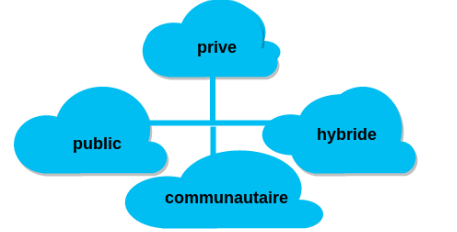
\includegraphics[scale=0.6]{Figures/modele_de_deployement.png}

\caption{figure : modele de deployement}
\label{fig3}
\end{center}
\begin{description}
 \item \textbf{Le Cloud priv�:}Un cloud priv� est une infrastructure de cloud n'est utilis� que par une seule organisation. Le cloud priv� peut �tre g�r�e par l'organisation elle-m�me ou par un prestataire de service qui peut �tre situ�e dans les locaux de l'organisation ou � l'externe chez le prestataire de services.
L'avantage suppl�mentaire du cloud priv� c'est contr�le total des donn�es par l'organisation, d'autre fa�on il permet la confidentialit� et la s�curit� des donn�es gr�ce aux ressources qui ne peuvent pas �tre partag�es par d'autre organisations[4].
 \item \textbf{Le Cloud communautaire�:}L'architecture est d�di�e � une communaut� professionnelle sp�cifique, pour permettre de travailler de mani�re collaborative sur un m�me projet.
 \item \textbf{Le Cloud public�:}Le cloud public est accessible publiquement � tous les particuliers et les groupe industriels. Son propri�taire est un fournisseur de service IaaS, PaaS ou SaaS. Les consommateurs ne sont factur�s que pour les applications, les services ou les donn�es qu'ils utilisent. Les ressources sont illimit�es et il n'y a donc aucun investissement initial. Les � Clouds � publics sont g�n�ralement exploit�s par des les fournisseurs de cloud commerciaux comme Amazon, Google, Microsoft, GoGrid.
 \item \textbf{Le Cloud hybride�:}Le cloud hybride est une composition de deux ou plusieurs infrastructures de Cloud publics et priv�s. G�n�ralement les donn�es sensibles sont g�r�es au niveau interne par l'organisation ou chez le prestataire de cloud prive et l'autre type de donn�es sont g�r�es par le cloud pu
\end{description}
\section{providers cloud computing�}
�l'existence du ��cloud computing��et et sa valeur pour les consommateurs sont aujourd'hui plus �videntes pour le grand public ,les  diff�rents acteurs du monde IT comme Google et Microsoft proposent des services de Cloud Computing.
�\begin{center}
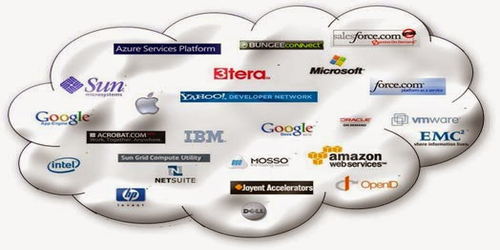
\includegraphics[scale=0.6]{Figures/cloud_providers.png}

\caption{figure : cloud provider}
\label{fig4}
\end{center}
 \subsection{Amazon :}� Amazon Web Services � (AWS) met � disposition un cloud public depuis 2006. Au d�part le but d'Amazon �tait de rentabiliser ses �normes infrastructures requises pour assumer les
mont�es en charge pendant la p�riode de No�l sur leur boutique en ligne.
Aujourd'hui Amazon propose de nombreux services en ligne, � commencer par l'IaaS probablement le plus connu : Elastic Compute Cloud (EC2).
\subsection{Salesforce :}Salesforce.com est une soci�t� qui a lanc� d�s 2003 des offres de Cloud public. C'est officiellement le plus ancien prestataire dans ce domaine. Aujourd'hui encore, leurs offres sont uniquement compos�es de Cloud Public, et adress�es aux entreprises (surtout les grands comptes). Les outils propos�s sont tourn�s vers le travail collaboratif, la gestion des ventes et le marketing relationnel.
\subsection{Google AppEngine�:}Google mise beaucoup sur le cloud computing et propose des services PaaS et SaaS.
A grande �chelle, les solutions de Google dans le cloud sont surtout connues des
consommateurs priv�s au travers des ses Google Apps telles que Google Docs, Calendar ou
encore Gmail. Toutes ces � web apps � sont dans le domaine du SaaS et gratuites pour une
utilisation priv�e.
Google App Engine dont la premi�re version beta est sortie en avril 2008 est le service PaaS
de Google. Au d�part le service ne supportait que le d�veloppement d'applications en
Python. Depuis, le support de Java Virtual Machines (JVMs) a �t� ajout� et permet de
d�velopper des applications non seulement en Java mais aussi au moyen de JRuby, JPython,
Scala ou Clojure. Le SDK (software development kit) inclut un environnement complet de
d�veloppement qui simule App Engine en local sur le bureau du d�veloppeur (Rhoton,
2010).
La plateforme inclut �galement des services sous formes d'API permettant de manipuler des
images, d'envoyer des mails ou encore d'utiliser les comptes Google pour les identifications au sein de l'application.

\subsection{Windows Azure�:}Windows Azure est une fondation pour ex�cuter des applications et stocker des donn�es dans un cloud. Elle fournit les logiciels que les clients de Microsoft peuvent installer et ex�cuter eux-m�mes sur leur propre ordinateur. Windows Azure est aujourd'hui un service, que les clients utilisent pour ex�cuter des applications et stocker des donn�es sur des machines accessibles par Internet appartenant � Microsoft. Ces applications peuvent fournir des services aux entreprises, aux consommateurs ou les deux. Windows Azure a �t� con�ue en partie au soutien de Microsoft applications SaaS, si les �diteurs de logiciels peuvent aussi l'utiliser commeune base pour une vari�t� de logiciels de clouds � vocation commerciale.
\section{Conclusion�: }Conclusion�: Le Cloud Computing se positionne actuellement en t�te de liste des nouvelles technologies. Il
se caract�rise par son extensibilit� et �lasticit� et son exploitabilit� par un grand nombre
d'utilisateurs dans le monde entier .il offre un grand   puissance de calcul et espace de stockage, comme toute innovation technologique qui se respecte, le nuage informatique fait �conomiser de
l'argent ,le cout ,le temp de utilisations des logiciel le developement et l'insatallaion.




\chapter{Conception}
\section{Introduction}



\section{Notions g�n�rales}

\subsection{Aspect syntaxique}
La syntaxe d'un langage est d�finie par un ensemble d'expressions (des mots, des phrases, des instructions, ou des diagrammes). Ces expressions peuvent �tre de deux types~: les expressions simples  et les expressions construites � partir d'autres expressions. Ainsi, pour exprimer une syntaxe d'un langage, on trouve plusieurs approches o� les deux les plus utilis�es sont l'approche par m�tamod�lisation et l'approche grammaticale. La syntaxe d'un langage peut �tre l'un des deux types suivants~:


\chapter{Impl�mentation}
\section{Introduction}



\section{Notions g�n�rales}

\subsection{Aspect syntaxique}
La syntaxe d'un langage est d�finie par un ensemble d'expressions (des mots, des phrases, des instructions, ou des diagrammes). Ces expressions peuvent �tre de deux types~: les expressions simples  et les expressions construites � partir d'autres expressions. Ainsi, pour exprimer une syntaxe d'un langage, on trouve plusieurs approches o� les deux les plus utilis�es sont l'approche par m�tamod�lisation et l'approche grammaticale. La syntaxe d'un langage peut �tre l'un des deux types suivants~:


\chapter*{Conclusion g�n�rale}

\end{spacing}
%-------------------------------------------------------------------
%                       La bibliographie
%-------------------------------------------------------------------
%\nocite{*}
%----------------------------
\bibliographystyle{plain}
\bibliography{Biblio}
%-------------------------------------------------------------------
%                       L'Annexe
%-------------------------------------------------------------------
%\begin{appendices}
%begin{appendices}
\end{document}
